%\VignetteIndexEntry{Processing of bead array data}
%\VignetteDepends{pixmap}
%\VignetteKeywords{beadarray, preprocessing}
%\VignettePackage{beadarray}

\documentclass[a4paper]{article}

\newcommand{\Robject}[1]{{\texttt{#1}}}
\newcommand{\Rfunction}[1]{{\texttt{#1}}}
\newcommand{\Rpackage}[1]{{\textit{#1}}}
\newcommand{\Rclass}[1]{{\textit{#1}}}
\newcommand{\Rmethod}[1]{{\textit{#1}}}
\newcommand{\Rfunarg}[1]{{\textit{#1}}}
\newcommand\pic[3]{\resizebox{#1}{#2}{\includegraphics{#3}}}

\usepackage{Sweave}

\begin{document}


\section{Introduction}
\label{intro}

There are two methods for describing the results of a BeadArray experiment. Firstly, we can use \emph{bead-level data} whereby the position and intensity of each individual bead on an array is known. The methods available for processing bead level data are discussed in: Dunning,M.J et al, Quality Control and Low-level Statistical Analysis of Illumina Beadarrays, Submitted.

\emph{Bead summary data} can also be used whereby a summary intensity for each bead type on an array is given. The summarised values for a particular bead type can then be compared 
between different arrays within an experiment.

Whilst the \Rpackage{beadarray} package includes methods for processing data of both kinds, bead summary data is far more widely available at the present time.  As such the methods described within this document focus exclusivly on dealing with bead summary data.

\section{Reading and analysing bead summary data}

Pre-processed bead summary data can be read directly into our library. The function used is \Rfunction{readBeadSummaryData} and requires a vector giving the names of text files as an input. Each text file can describe the bead summary data for a particular array in the experiment, or it may describe all 96 experiments. Example files are provided at the following URL: 

 www.damtp.cam.ac.uk/user/jcm68/beadarray.html

Once the example files have been downloaded they can be read into {\sf R}. By default, the files are read from the current working directory in R, but this can be changed by setting the \Rfunarg{path} parameter. The \Robject{targets} object is used to define a vector of filenames to be read and is created by reading the beadSummaryTargets.txt file (see example file). For experiments with a large number of arrays, it may be inconvenient to create the text file. Therefore, the \Rfunction{readBeadSummaryData} is able to read all files in the working directory if the \Rfunarg{targets} parameter is omitted. By default, the function looks for each of the column headings as they are listed below. It is possible to use alternative names for headings (eg nobeads instead of NoBeads). For more details on this please see the appropriate help file.


\begin{itemize}
\item{SAMPLE - an identifier for the sample on the array}
\item{ProbeID - an each identifier for each bead type (probe type) on the array}
\item{AvgSig - Summary intensity produced by averaging bead intensities of all beads of a particular type}
\item{BeadStDev - Standard deviation of all beads of a particular type, outliers excluded}
\item{NoBeads - Number of beads used to produce average}
\item{Detection - Average detection score for each bead type}
\end{itemize}

A common cause of error when reading files is for the column names found in the files to not match the headings that {\sf R} expects to find. The \Rfunction{readBeadSummaryTargets} function prints out the name of the file being read and also the first line of the file. 
This shows the column names present in the file and will help to identify problems. Usage of \Rfunction{readBeadSummaryTargets} is as follows:

\begin{Schunk}
\begin{Sinput}
> targets = readBeadSummaryTargets()
> BSData = readBeadSummaryData(targets)
> BSData
\end{Sinput}
\end{Schunk}


The resulting object, a \Rclass{BeadSummaryList}, is a list based object with the following sublists: 

\begin{itemize}
\item{R - averaged foreground intensities}
\item{Rb - averaged background intensities}
\item{probeID - unique identifer for the probe}
\item{beadstdev - standard deviation of all beads of a particular type}
\item{nobeads - number of beads used to produce average}
\item{Detection - average detection score for each bead type}
\item{SAMPLE - identifier for the sample}
\item{SAM - identifier for the SAM that the array was part of}
\end{itemize}

The first 6 entries in a \Rclass{BeadSummaryList} are all matrices with the each row corresponding to a particular bead type and the columns to individual arrays.  The final two entries are vectors with each entry holding details related to a specific array. \\

All functions described from now on use a \Rclass{BeadSummaryList} object as a parameter. This object can either be created using the steps described above, or can be created from bead-level data by using 
the \Rfunction{createBeadSummaryData} function (see Dunning et al).

We can use the detection score as a preliminary indicator of the quality of each array.  Using the following commands we can construct a boxplot of the detection scores for each probe.  If the scores look low then it would advisable to take a closer look at the array in order to identify a reason, e.g. a bad hybridization. Boxplots of the\Robject{ R} and \Robject{Rb} columns can also be informative.

\begin{center}
\begin{Schunk}
\begin{Sinput}
> boxplot((BSData$Detection) ~ col(BSData$Detection), main = "Detection Scores")
\end{Sinput}
\end{Schunk}
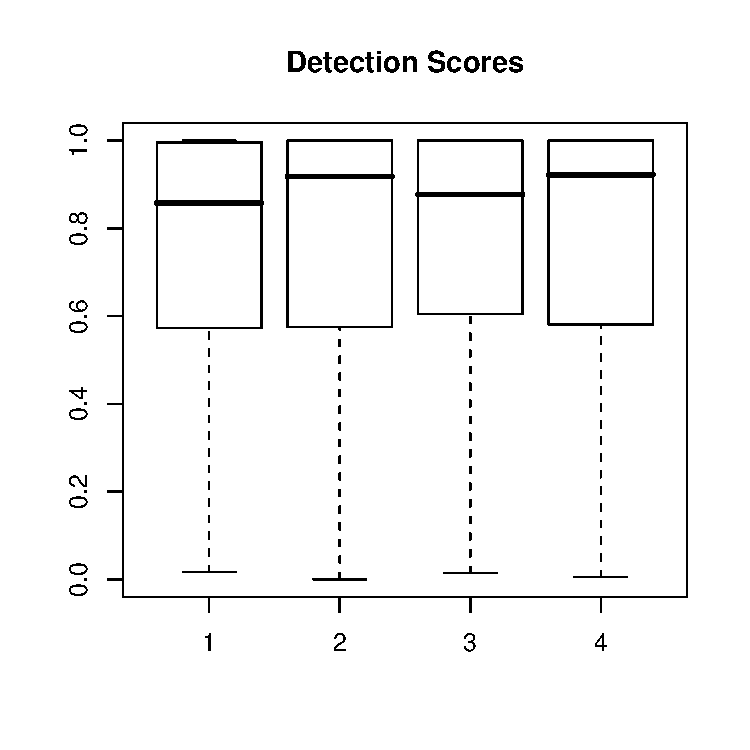
\includegraphics{bead-vignette-31}
\end{center}



\section{Plotting Values Across Whole SAMs and Use of Control Information}
\label{plotting_across_arrays}

We have provided a SAM summary plot for when we want to compare the intensity of a particular bead type across all arrays on one SAM. In its most simple form we use \Rfunction{plotOnSAM(v)} where \Robject{v}
is simply a vector of numeric values with length 96. To create the vector \Robject{v} we could make use of the function \Rfunction{getMeanIntensities(BSData, probe)} which will return the mean intensity of beads with probeID on each of the
arrays in the experiment. For instance probeID 4279 is a housekeeping control in the example experiment, so we can do.

\begin{Schunk}
\begin{Sinput}
> getMeanIntensities(BSData, 4279)
\end{Sinput}
\end{Schunk}

As an example we show the variation in a hybridisation control across 96 arrays

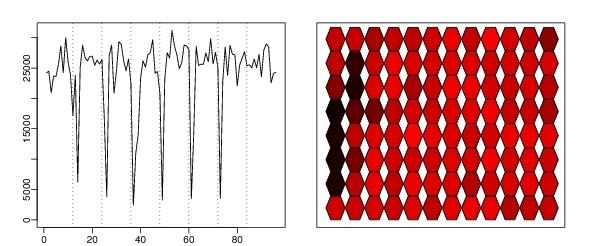
\includegraphics{testpdf2.jpg}

On the left-hand plot we have array index on the x axis and on the y axis we have the corresponding value of v for each of the 96 arrays. Instantly we can see the numbers of arrays for which the value of \Robject{v} is lower.

On the right-hand plot we relate the vector \Robject{v} to the position of each array on the SAM. The arrays are numbered from 1 in top-left corner to 96 in the bottom-right corner. The colour of each hexagon is related to its value of \Robject{v}, the higher this value the brighter the shade of red (a greyscale version of the plot can also be made). 

In the figure above we can see that the line in the left hand plot is very erratic and the colour of the hexagons range from black through to bright red.  Both of these indicate that the values in vector \Robject{v} change greatly across the SAM.  Using the right hand plot we can quickly identify which probes have the lowest intensities allowing us to easily go and investigate the possible reasons. The BeadStudio application provided by Illumina is able to produce the plot seen in the left panel of the \Rfunction{plotOnSAM} function output, but we feel that our method is more flexible. With our function we can plot values of any 
probe (not just controls) and can plot intensities on both raw and logged scale. We can also see whereabouts any potential problem arrays are located on the SAM. In the examples above we found the values of a particular bead type across all arrays and used as input to \Rfunction{plotOnSAM}. This plotting function is flexible because it allows any vector of numeric values with length 96 as input. For instance we could also use the number of outliers on each of the 96 arrays or the number of unregistered beads as input. 
The \Rfunction{plotOnSAM} function is currently only appropriate for SAM technology where 96 BeadArrays are investigated simultaneously. A similar method is being developed for BeadChip technologies and will appear in the next version of \Rpackage{beadarray}.

\section{Comparing Samples}
\label{comparing_samples}

Now that all the arrays in the experiment have been averaged, we can see how particular bead types vary between different arrays or samples. We have implemented both XY plots and MA plots to achieve this.
In an XY plot, for a particular gene, we simply plot the value obtained from two different samples against each other with one sample on the x axis and one sample on the y axis. For an MA plot we plot the average intensity 
of each gene from the two different samples against the difference. For conventional microarrays, the MA plot can often reveal important differences between the two dyes used for hybridisation and give us an idea of the 
amount of noise generated by experiments. 

The functions created for the library are capable of making comparisons between the red and green channels for the same array as well as between two arrays from a one-colour experiment. However, we did not have any two 
colour data when creating this document, so the following examples will be for comparing two different arrays from a one-colour experiment.


We might want to know about the variation between replicates of the same sample in an experiment. The function \Rfunction{pairwiseMA} is capable of producing XY plots and MA plots for a defined set of arrays with XY and MA plots shown for all pairwise comparisons between the arrays

In our experiment arrays 1,2,3 \& 4 were replicates of the same sample.

\begin{center}
\begin{Schunk}
\begin{Sinput}
> vec = c(1, 2, 3, 4)
> pairwiseMA(BSData, vec)
\end{Sinput}
\end{Schunk}

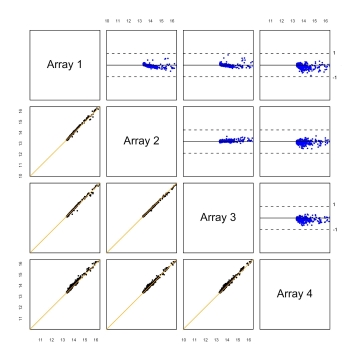
\includegraphics{pairwise2.jpg}

\end{center}

The resulting graphic is in a 4 x 4 grid. In the first row we have MA-plots of the first array compared to arrays 2,3 and 4 and in the first column there are XY plots of the first array compared to arrays 2,3 and 4. 

As we are comparing replicates of the sample we would expect to see very little variation in the plots so XY plots should be centred around the diagonal and MA plots about the horizontal

The normalisation methods used for bead-level data (median and quantile), can also be applied to bead summary data. An additional normalisation method exists for the normalisation of bead summaries. This is known as \emph{qspline normalisation} and uses quantiles from each array and a target distribution to fit a smoothing function to each array. 

\begin{Schunk}
\begin{Sinput}
> BSData.qsp = qsplineNormalise(BSData)
\end{Sinput}
\end{Schunk}

\end{document}
